
%% bare_jrnl.tex
%% V1.4b
%% 2015/08/26
%% by Michael Shell
%% see http://www.michaelshell.org/
%% for current contact information.
%%
%% This is a skeleton file demonstrating the use of IEEEtran.cls
%% (requires IEEEtran.cls version 1.8b or later) with an IEEE
%% journal paper.
%%
%% Support sites:
%% http://www.michaelshell.org/tex/ieeetran/
%% http://www.ctan.org/pkg/ieeetran
%% and
%% http://www.ieee.org/

%%*************************************************************************
%% Legal Notice:
%% This code is offered as-is without any warranty either expressed or
%% implied; without even the implied warranty of MERCHANTABILITY or
%% FITNESS FOR A PARTICULAR PURPOSE! 
%% User assumes all risk.
%% In no event shall the IEEE or any contributor to this code be liable for
%% any damages or losses, including, but not limited to, incidental,
%% consequential, or any other damages, resulting from the use or misuse
%% of any information contained here.
%%
%% All comments are the opinions of their respective authors and are not
%% necessarily endorsed by the IEEE.
%%
%% This work is distributed under the LaTeX Project Public License (LPPL)
%% ( http://www.latex-project.org/ ) version 1.3, and may be freely used,
%% distributed and modified. A copy of the LPPL, version 1.3, is included
%% in the base LaTeX documentation of all distributions of LaTeX released
%% 2003/12/01 or later.
%% Retain all contribution notices and credits.
%% ** Modified files should be clearly indicated as such, including  **
%% ** renaming them and changing author support contact information. **
%%*************************************************************************


% *** Authors should verify (and, if needed, correct) their LaTeX system  ***
% *** with the testflow diagnostic prior to trusting their LaTeX platform ***
% *** with production work. The IEEE's font choices and paper sizes can   ***
% *** trigger bugs that do not appear when using other class files.       ***                          ***
% The testflow support page is at:
% http://www.michaelshell.org/tex/testflow/

\documentclass[10pt,journal,compsoc]{IEEEtran}
%
% If IEEEtran.cls has not been installed into the LaTeX system files,
% manually specify the path to it like:
% \documentclass[journal]{../sty/IEEEtran}



% *** CITATION PACKAGES ***
%
%\ifCLASSOPTIONcompsoc
  % IEEE Computer Society needs nocompress option
  % requires cite.sty v4.0 or later (November 2003)
  \usepackage[nocompress]{cite}

% *** GRAPHICS RELATED PACKAGES ***
\usepackage{graphicx}
\graphicspath{ {./images/} }


% *** MATH PACKAGES ***
%
\usepackage{amsmath}
% A popular package from the American Mathematical Society that provides
% many useful and powerful commands for dealing with mathematics.
%
% Note that the amsmath package sets \interdisplaylinepenalty to 10000
% thus preventing page breaks from occurring within multiline equations. Use:
%\interdisplaylinepenalty=2500
% after loading amsmath to restore such page breaks as IEEEtran.cls normally
% does. amsmath.sty is already installed on most LaTeX systems. The latest
% version and documentation can be obtained at:
% http://www.ctan.org/pkg/amsmath



% *** SPECIALIZED LIST PACKAGES ***
%
%\usepackage{algorithm,algorithmic}
\usepackage[ruled,vlined,linesnumbered]{algorithm2e}
% algorithmic.sty was written by Peter Williams and Rogerio Brito.
% This package provides an algorithmic environment fo describing algorithms.
% You can use the algorithmic environment in-text or within a figure
% environment to provide for a floating algorithm. Do NOT use the algorithm
% floating environment provided by algorithm.sty (by the same authors) or
% algorithm2e.sty (by Christophe Fiorio) as the IEEE does not use dedicated
% algorithm float types and packages that provide these will not provide
% correct IEEE style captions. The latest version and documentation of
% algorithmic.sty can be obtained at:
% http://www.ctan.org/pkg/algorithms
% Also of interest may be the (relatively newer and more customizable)
% algorithmicx.sty package by Szasz Janos:
% http://www.ctan.org/pkg/algorithmicx




% *** ALIGNMENT PACKAGES ***
%
\usepackage{array}
% Frank Mittelbach's and David Carlisle's array.sty patches and improves
% the standard LaTeX2e array and tabular environments to provide better
% appearance and additional user controls. As the default LaTeX2e table
% generation code is lacking to the point of almost being broken with
% respect to the quality of the end results, all users are strongly
% advised to use an enhanced (at the very least that provided by array.sty)
% set of table tools. array.sty is already installed on most systems. The
% latest version and documentation can be obtained at:
% http://www.ctan.org/pkg/array


% *** SUBFIGURE PACKAGES ***
%\ifCLASSOPTIONcompsoc
%  \usepackage[caption=false,font=normalsize,labelfont=sf,textfont=sf]{subfig}
%\else
  \usepackage[caption=false,font=footnotesize]{subfig}
%\fi
% subfig.sty, written by Steven Douglas Cochran, is the modern replacement
% for subfigure.sty, the latter of which is no longer maintained and is
% incompatible with some LaTeX packages including fixltx2e. However,
% subfig.sty requires and automatically loads Axel Sommerfeldt's caption.sty
% which will override IEEEtran.cls' handling of captions and this will result
% in non-IEEE style figure/table captions. To prevent this problem, be sure
% and invoke subfig.sty's "caption=false" package option (available since
% subfig.sty version 1.3, 2005/06/28) as this is will preserve IEEEtran.cls
% handling of captions.
% Note that the Computer Society format requires a larger sans serif font
% than the serif footnote size font used in traditional IEEE formatting
% and thus the need to invoke different subfig.sty package options depending
% on whether compsoc mode has been enabled.


% *** PDF, URL AND HYPERLINK PACKAGES ***
%
\usepackage{url}
% url.sty was written by Donald Arseneau. It provides better support for
% handling and breaking URLs. url.sty is already installed on most LaTeX
% systems. The latest version and documentation can be obtained at:
% http://www.ctan.org/pkg/url
% Basically, \url{my_url_here}.

\usepackage{hyperref}


% *** Do not adjust lengths that control margins, column widths, etc. ***
% *** Do not use packages that alter fonts (such as pslatex).         ***
% There should be no need to do such things with IEEEtran.cls V1.6 and later.
% (Unless specifically asked to do so by the journal or conference you plan
% to submit to, of course. )

%Alessandro input: makecell package to permite line break inside tables
\usepackage{makecell}
\usepackage{xcolor}
% correct bad hyphenation here
\hyphenation{op-tical net-works semi-conduc-tor}
\usepackage{lscape}
%\renewcommand{\baselinestretch}{0.975}

\begin{document}
%
% paper title
% Titles are generally capitalized except for words such as a, an, and, as,
% at, but, by, for, in, nor, of, on, or, the, to and up, which are usually
% not capitalized unless they are the first or last word of the title.
% Linebreaks \\ can be used within to get better formatting as desired.
% Do not put math or special symbols in the title.
%\title{Building a framework to perform automated verification of solar photovoltaic off-grid systems}
\title{Multi-core synthesis and maximum satisfiability applied to obtain optimal sizing of solar photovoltaic systems}
%
%
% author names and IEEE memberships
% note positions of commas and nonbreaking spaces ( ~ ) LaTeX will not break
% a structure at a ~ so this keeps an author's name from being broken across
% two lines.
% use \thanks{} to gain access to the first footnote area
% a separate \thanks must be used for each paragraph as LaTeX2e's \thanks
% was not built to handle multiple paragraphs
%

\author{Edilson Galvão, Alessandro~Trindade and Lucas~Cordeiro% <-this % stops a space
\IEEEcompsocitemizethanks{
\IEEEcompsocthanksitem{E. Galvão is with MSc student in the Post-graduate Program in Electrical Engineering, Manaus, Brazil, e-mail: esj.galvao@gmail.com.}
\IEEEcompsocthanksitem{A. Trindade is with the Department of Electricity, Federal University of Amazonas, Manaus, Brazil, e-mail: alessandrotrindade@ufam.edu.br.}% <-this % stops a space
\IEEEcompsocthanksitem{L. Cordeiro is with School of Computer Science, The University of Manchester, UK, e-mail: lucas.cordeiro@manchester.ac.uk.}}% <-this % stops a space
%\thanks{The authors would like to thank ????, for the financial support.}
\thanks{This study was financed in part by the Coordenação de Aperfeiçoamento de Pessoal de Nível Superior - Brasil (CAPES) - Finance Code 001.}
\thanks{Manuscript received March XX, 2021; revised XXXXX 11, 2021.}}

% note the % following the last \IEEEmembership and also \thanks - 
% these prevent an unwanted space from occurring between the last author name
% and the end of the author line. i.e., if you had this:
% 
% \author{....lastname \thanks{...} \thanks{...} }
%                     ^------------^------------^----Do not want these spaces!
%
% a space would be appended to the last name and could cause every name on that
% line to be shifted left slightly. This is one of those "LaTeX things". For
% instance, "\textbf{A} \textbf{B}" will typeset as "A B" not "AB". To get
% "AB" then you have to do: "\textbf{A}\textbf{B}"
% \thanks is no different in this regard, so shield the last } of each \thanks
% that ends a line with a % and do not let a space in before the next \thanks.
% Spaces after \IEEEmembership other than the last one are OK (and needed) as
% you are supposed to have spaces between the names. For what it is worth,
% this is a minor point as most people would not even notice if the said evil
% space somehow managed to creep in.



% The paper headers
\markboth{IEEE Transactions on Computers,~Vol.~XX, No.~YY, January~2021}%
{Trindade \MakeLowercase{\textit{et al.}}: Multi-core synthesis and maximum satisfiability applied to obtain optimal sizing of solar photovoltaic systems}
% The only time the second header will appear is for the odd numbered pages
% after the title page when using the twoside option.
% 
% *** Note that you probably will NOT want to include the author's ***
% *** name in the headers of peer review papers.                   ***
% You can use \ifCLASSOPTIONpeerreview for conditional compilation here if
% you desire.




% If you want to put a publisher's ID mark on the page you can do it like
% this:
%\IEEEpubid{0000--0000/00\$00.00~\copyright~2015 IEEE}
% Remember, if you use this you must call \IEEEpubidadjcol in the second
% column for its text to clear the IEEEpubid mark.



% use for special paper notices
%\IEEEspecialpapernotice{(Invited Paper)}

% As a general rule, do not put math, special symbols or citations
% in the abstract or keywords.
\IEEEtitleabstractindextext{%
\begin{abstract}
Given that annual global energy consumption growth is around $1.3$\% with forecasts until $2040$; photovoltaic systems become a suitable alternative to traditional means of generating energy such as nuclear and fossil. To promote this technology's dissemination and expand the use of renewable energies, we describe and evaluate an automated formal synthesis approach that assists in decision-making when implementing an off-grid residential system. Our proposed approach, called PVz, can obtain the optimal sizing of photovoltaic systems focusing on Life Cycle Cost (LCC) analysis. Given the electrical needs of a home, we seek a large set of electrical equipment with the best possible combination of devices for synthesizing renewable energy systems that meet the specified energy demand. Also, we calculate all costs related to maintenance, such as equipment replacement, system operation, and general maintenance over $20$ years. The results presented here are based on seven case studies that denote different energy consumptions. The same case studies were solved by a commercial optimization tool. Our technique and the commercial tool results were validated with another commercial design software to perform a fair comparison. Furthermore, we analyze some topics such as runtime, optimal solution, and configuration of the resulting systems. We claim that our technique is advantageous compared to the tools for photovoltaic sizing and optimization available on the market.
\end{abstract}

% Note that keywords are not normally used for peerreview papers.
\begin{IEEEkeywords}
Formal synthesis, software verification, model checking, solar photovoltaic systems.
\end{IEEEkeywords}}

% make the title area
\maketitle

% For peer review papers, you can put extra information on the cover
% page as needed:
% \ifCLASSOPTIONpeerreview
% \begin{center} \bfseries EDICS Category: 3-BBND \end{center}
% \fi
%
% For peerreview papers, this IEEEtran command inserts a page break and
% creates the second title. It will be ignored for other modes.
\IEEEpeerreviewmaketitle



\IEEEraisesectionheading{\section{Introduction}}
% The very first letter is a 2 line initial drop letter followed
% by the rest of the first word in caps.
% 
% form to use if the first word consists of a single letter:
% \IEEEPARstart{A}{demo} file is ....
% 
% form to use if you need the single drop letter followed by
% normal text (unknown if ever used by the IEEE):
% \IEEEPARstart{A}{}demo file is ....
% 
% Some journals put the first two words in caps:
% \IEEEPARstart{T}{his demo} file is ....
% 
% Here we have the typical use of a "T" for an initial drop letter
% and "HIS" in caps to complete the first word.
--------------------
 
\IEEEPARstart{T}{he} recent studies about global energy indicate that $789$ million people have no access to electricity, which is $10$\% of the world population~\cite{Energyprogressreport}. From $2010$ until $2018$, the effort to reduce the number of people without electricity access increased, and the result is positive. Quantitatively the result was a decrease from $1.2$ billion to $0.84$ billion people without electrical energy. Out of this total, renewable energy solutions are responsible for $136$ million people receiving basic energy service~\cite{Energyprogressreport}. Unfortunately, lack of access to clean and affordable energy is considered a core dimension of poverty~\cite{Hussein2012}; this has a direct impact on the low Human Development Index (HDI) of different localities~\cite{Coelho}. It follows that increased access to energy allows economic growth and poverty alleviation\cite{Karekesi}. 

To provide electricity for all, decentralized systems led by solar photovoltaic (PV) in off-grid and mini-grid systems will be the lowest-cost solution for three-quarters of the connections needed~\cite{Hussein2012}. Thus, this can be ratified by analyzing the result of renewable energy reported by the global bank, where $17.3$\%  of global energy is based on wind and solar energy~\cite{Energyprogressreport}.

Changes to improve the electrical energy uses, the more precise the sizing for electrical grids or stand-alone systems, the more meaningful the use of renewable energies. For this purpose, some software is available in the market; a part of them is created for general-purpose as MATLAB~\cite{Benatiallah2017} and others for specific electrification studies like RETScreen, and HOMER~\cite{Pradhan,Swarnkar}. However, the industry demands the design solution to be the optimum, considering equipment manufacturers and models available on the market and not just minimum or maximum values of current or power for the optimized items \textcolor{red}{add citation}. We need to evaluate the electrical compatibility among the equipment, which can only be achieved with specialized PV optimization software. Therefore, the optimal solution is the lowest cost from a list of equipment that meets the house's electrical demands.

Given the above, the HOMER tool manages to deliver an optimal solution in a smaller scope, where only batteries and solar panels are optimized, while all other modules are simulated. In contrast, the technique described in this work, called PVz, is capable of optimizing, in addition to solar panels and batteries, electrical inverters, and controllers. The clear difference between the optimized electrical devices ensures greater assertiveness once both techniques are compared, thus favoring more extensive design-space coverage.

Here, we have developed a variant of the counterexample guided inductive synthesis (CEGIS)~\cite{AbateCAV2018} for synthesizing optimal sizing of stand-alone PV systems using commercial equipment data. If the user gives a correctness specification $\sigma$, our technique uses that as a starting point and then iteratively produces a sequence of candidate solutions that satisfy $\sigma$, related to power reliability.
 
We used a solver called Z3 \textcolor{red}{add citation}. Internally, the Z3 tool contains a module to include optimization objectives. This module is named $\nu$Z and integrates state-of-the-art algorithms for optimization and extra tools to solve linear restrictions problems. In particular, the $\nu$Z features match our problem and will help us to optimize PV systems~\cite{BjornerPF15}. In each iteration, we synthesize the sizing of stand-alone PV systems, but that may not achieve the lowest cost. Thus, the candidate solution passes through an SMT solver to reduce the number of possible states. Our candidate solution provides a lower bound, which serves as the minimum cost of reference to help our engine restrict verification. Note that each iteration can be lower or higher than the current reference, once found a value lower than the current reference, and it respects the user constraints. The reference is updated globally. If the verification by the SMT solver step does fail, it means there is an optimal solution. Thus, all content produced is saved as a counterexample with an optimal sizing that meets both power reliability and system cost. If the verification step does not fail, the content produced is ignored. Our novelty relies on a practical approach to pursuing the optimal solution of PV systems using formal methods. 

Research in the fields of renewable energy and photovoltaic systems, date from the mid-90s, and bring different approaches to find an optimal solution for the design of electrical systems as can be seen in~\cite{Driouich2018} and~\cite{Applasamy2011}. However, the amount of work related to the formal modeling of photovoltaic systems is still low. Consequently, it is even more challenging to find work based on modern solvers \textcolor{red}{what do you mean by modern solvers?}. The starting point for this work~\cite{VSTTE2020}~\cite{TrindadeCordeiro19} are studies that derive from the year $2019$ and converge to analyze the optimization problem of photovoltaic systems using SMT solvers and commercial tools such as HOMER and PVsyst. 

This paper makes the following original contributions. First, it is a radical improvement in the base paper's performance describing formal synthesis for stand-alone PV systems application \textcolor{red}{add citation}. Second, the technique described here supports data processing parallelization since it relies on a multi-core processor. Third, the state space coverage was increased compared to the base article~\cite{VSTTE2020}. It was possible to cover and compute all the spaces of the combinations of electrical equipment. Fourth, experimental results with seven case studies show that the formal synthesis approach qualitatively outperforms an existing state-of-the-art optimization tool. Lastly, the results are validated with accurate commercial design software called PVsyst.

%-----------------------------------------------------------
\section{Background}
\label{sec:AutomatedVerification}
%-----------------------------------------------------------
 
Fig.~\ref{fig:optimization} illustrates how to obtain the optimal sizing of a stand-alone PV system using two different modes. The first one is the traditional model called \textit{\textbf{traditional sizing}}, which includes manual verification by computing the electrical equipment capacity and installation for validation. Concerning the first mode, there are still commercial tools as MATLAB~\cite{Benatiallah2017} and Homer~\cite{Pradhan,Swarnkar}, which simulate the real electrical system. The second includes \textbf{\textit{Automated Synthesis}} that encompasses verification engines. This option proves to be viable since it generates more complex and accurate data than the traditional way described previously. Both modes described here use the same input and theoretically produce the same output; it is noteworthy that variables such as electrification, support for different categories of equipment, and different electrical sizing forms impact the expected output.

For \textbf{input} data, we can consider weather data, price information about each piece of equipment, design requirements, load curve, power demand, and design assumptions. This information is converted into a matrix of data and exposed as global content to the software.

For the \textbf{output} data and a more straightforward reading of this work, we will assume from now on that every benchmark that contains a valid answer will be called \textbf{satisfiable (SAT)}. By contrast, when there is no solution, we will call it \textbf{unsatisfiable (UNSAT)}. If there is a set of renewable energy equipment, which can be combined (price and system hardware composition), then the result is SAT.
%
\begin{figure}[h]
\fbox{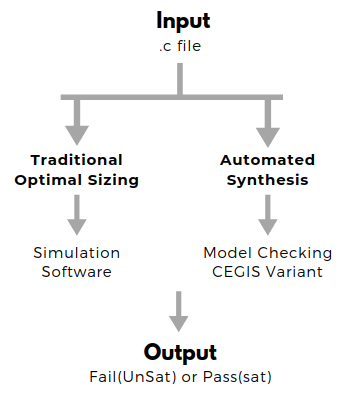
\includegraphics[width=0.38\textwidth]{TraditonalVsAutoFlow.png}}
\centering
\caption{Comparative image of the traditional method versus the proposed method.}
\label{fig:optimization}
\end{figure}
  
Note that the automated synthesis technique is a mathematical reasoning about a formal model, where the SAT result is a counterexample with detailed information on the optimal solution \textcolor{red}{what is a counterexample? we need to define here}. Thus, the answer can guide the software or client to choose the best combination of electrical machines. The traditional way does not offer the quantity of necessary data about the system and internal modes \textcolor{red}{add citation}. Another notable topic that needs to highlight is about each model's coverage; models that use automated kernel \textcolor{red}{what do you mean by automated kernel?} can ensure a complete coverage over the entire state-space, instead of locals states as a traditional model \textcolor{red}{this last sentence is unclear}. 

%-----------------------------------------------------------
\subsection{Program Synthesis}
\label{sec:ProgramSynthesis}
%-----------------------------------------------------------

The basic idea of program synthesis is to automatically construct a $P$ program that satisfies a correctness specification $\sigma$. In particular, program synthesis is automatically performed by engines that use a correctness specification $\sigma$, as a starting point and then incrementally produce a sequence of candidate solutions that partially satisfy $\sigma$~\cite{Abateetal2017}. As a result, a given candidate program $p$ is iteratively refined to match $\sigma$ more closely. Figure~\ref{Counter-Example-Guided-Inductive-Synthesis} illustrates the underlying architecture. 
%
\begin{figure}[h]
\begin{center}
\fbox{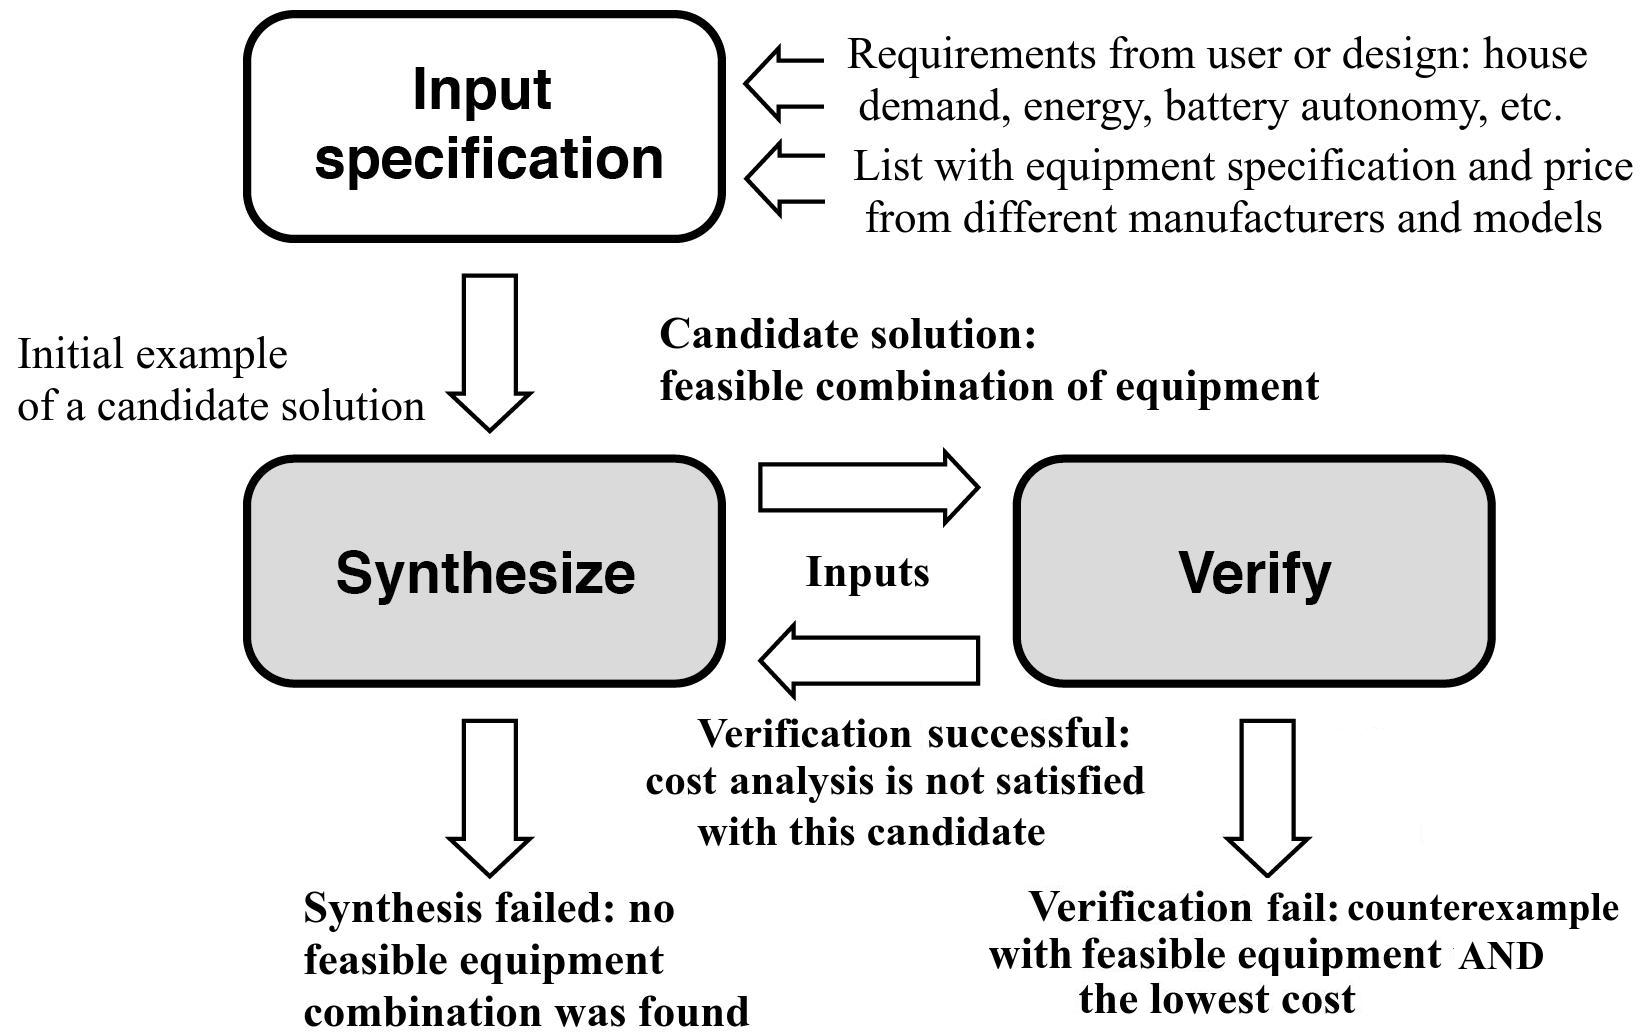
\includegraphics[width=0.47\textwidth]{fig2_rev2.jpg}}
\end{center}
	\caption{CEGIS in PV system sizing.}
	\label{Counter-Example-Guided-Inductive-Synthesis}
\end{figure}

The correctness specification $\sigma$ provided to our synthesizer is of the form $\exists \vec{F}. \forall \vec{x}. \sigma(\vec{x}, \vec{F})$, where $\vec{F}$ ranges over functions, $\vec{x}$ ranges over ground terms, and $\sigma$ is a quantifier-free (QF) formula typically supported by SMT solvers. The ground terms are interpreted over some finite domain $\mathcal{D}$, where $\mathcal{D}$ can be encoded using the SMT's bit-vectors part. Our specification includes house demand, energy, and battery autonomy; we also provide equipment specifications and prices from different manufacturers and models.

In Figure~\ref{Counter-Example-Guided-Inductive-Synthesis}, the phases {\sc Synthesize} and {\sc Verify} interact via a finite set of test vectors {\sc inputs}, which is incrementally updated. Given the correctness specification $\sigma$, the {\sc Synthesize} procedure tries to find an existential witness $\vec{F}$ satisfying the specification $\sigma(\vec{x}, \vec{F})$, for all $\vec{x}$ in {\sc inputs} (as opposed to all $\vec{x} \in \mathcal{D}$). If {\sc Synthesize} succeeds in finding a witness~$\vec{F}$, the latter is a candidate solution to the full synthesis formula, which is passed to {\sc Verify} to check whether it is a proper solution ({\it i.e.}, $\vec{F}$ satisfies the specification $\sigma(\vec{x}, \vec{F})$ for all $\vec{x}\in\mathcal{D}$). If this is the case, then the algorithm terminates.

One may notice that each iteration of the traditional CEGIS loop adds a new input to the finite set $INPUTS$, which is then used for synthesis. Given that the full set of inputs $\mathcal{D}$ is finite because we use bit-vector expressions, the refinement loop can only iterate over a finite number of times. However, {\sc Synthesize} may conclude that no candidate solution obeying $\sigma$ for the finite set $INPUTS$ exists. 

In our CEGIS variant, there exist four differences related to the traditional one: 
(1) there exists no test vector, and every candidate is generated in the {\sc Synthesize} phase and sent to the {\sc Verify} phase; 
(2) if the {\sc Verify} phase is unsuccessful, then a new candidate is generated by {\sc Synthesize} and 
(3) the lower bound of the {\sc Verify} phase is incremented to search for the lowest cost; as a result,
(4) there exists no refinement from the {\sc Verify} phase back to the {\sc Synthesize} phase. In particular, a new counterexample is not added to the {\sc input} set since a failure during the {\sc Verify} phase will only discard a given candidate, which could be feasible in the next iteration with a new lower bound.

In summary, our proposal is a technique based on CEGIS, which aims to synthesize the optimal solution of a PV system; therefore, our technique addresses an optimization problem.

%%%%%%%%%%%%%%%%%%%%%%%%%%%%%%%%%%%%%%%%%%%%%%%%%%%%%%%%
\subsection{Sizing Stand-alone Solar PV Systems}
\label{sec:sizing}
%%%%%%%%%%%%%%%%%%%%%%%%%%%%%%%%%%%%%%%%%%%%%%%%%%%%%%%%

A PV system is illustrated in Fig.\ref{fig:blockdiagram}. It employs the PV generator (\textit{panel or an array}), a semiconductor device that can convert solar energy into DC electricity. We hold \textit{batteries}, where power can be stored and used for night hours or rainy days. The use of batteries as a storage form implies a \textit{charge controller}~\cite{Hansen}. The PV arrays produce DC, and therefore when the PV system contains an AC load, a DC/AC conversion is required (\textit{inverter}). The \textit{AC load} dictates the AC electrical load's behavior from the house that the system will feed.
%
\begin{figure}[h]
\fbox{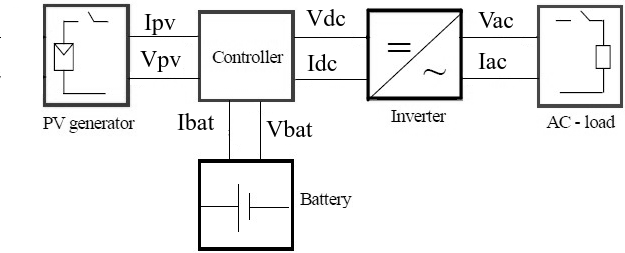
\includegraphics[width=0.47\textwidth]{blockdiagramPVS2_rev}}
\centering
\caption{Block diagram for a typical stand-alone PV system~\cite{Hansen}.}
\label{fig:blockdiagram} 
\end{figure}

The sizing check stage can ensure that the system meets the standard project steps related to the critical period method (worst month) for solar energy system sizing~\cite{Pinho}. It adopts an MPPT (Maximum Power Point Tracking) charge controller, which is the most common in use. 

Since this paper's audience is targeted to be from the software verification area, we decided to use a higher-level explanation about the PV sizing. The sizing process involves eighteen equations related to the electrical engineering area, which is detailed online.\footnote{\href{https://cutt.ly/Dz1Ua6Q}{https://cutt.ly/Dz1Ua6Q}} Fig.~\ref{fig:flow} illustrates the overview of the steps that must be taken to size a stand-alone PV system.
%
\begin{figure}[h]
\fbox{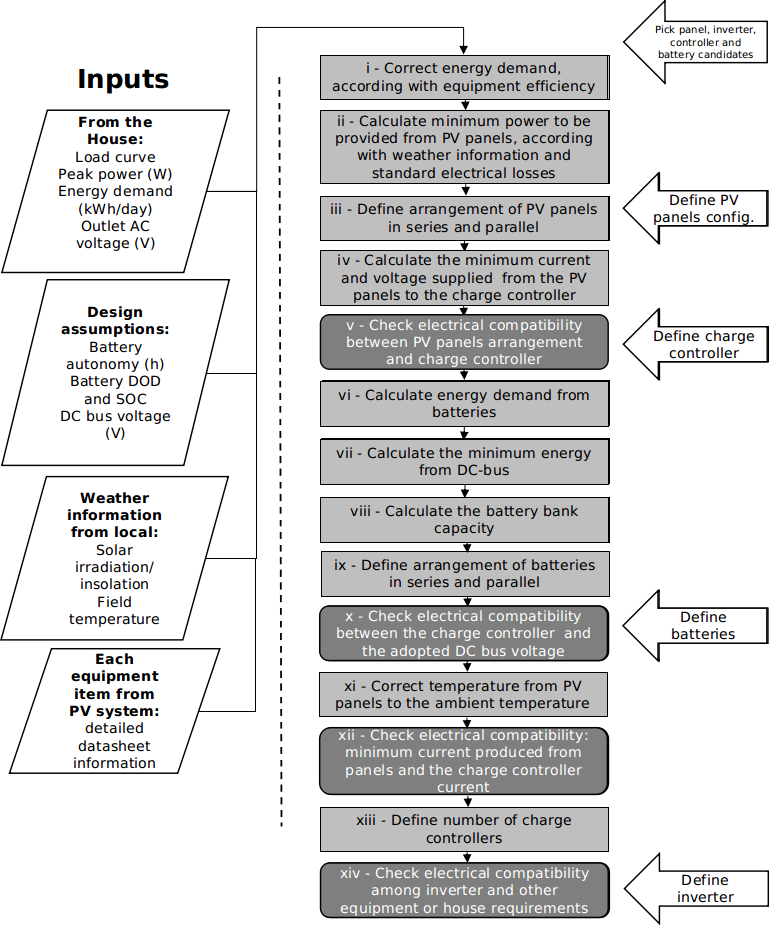
\includegraphics[width=0.47\textwidth]{flowchart}}
\centering
\caption{High level description of stand-alone PV system sizing process.}
\label{fig:flow} 
\end{figure}

On the left side of Fig.~\ref{fig:flow}, we describe the needed \textbf{inputs} to size a PV system. There are requirements from the house to be electrified; in particular, we have the design assumptions, weather information from the targeted local of the PV system deployment, and a possible initial list of equipment to be used, covering all the items listed Fig.\ref{fig:blockdiagram}. Concerning the equipment list, the designer can use a few pieces of equipment or a vast one. We can also decide not to adopt the commercial equipment list. However, the result is a PV sizing of specific power, current, or voltage values, usually just close to original equipment, found in the market. This possibility has the drawback of possible incompatibility among equipment when the real one is bought and deployed.

There exist specific steps that aim the calculation of some variables and others related to the electrical compatibility validation among equipment items, both enumerated from \textbf{i} to \textbf{xiv}, as illustrated in Fig.~\ref{fig:flow}; those represent different shades of gray of the rectangle boxes. The start point is usually a candidate list of PV panels, charge controller, battery, and inverter, as indicated at the top of the flowchart. The arrows on the right side show a point where some specific item is validated. The diagram does not show the returning location. However, if the candidate item is not compatible with others or does not meet some requirements, it must be changed to follow the indicated flow. The last rectangle box checks the inverter electrical compatibility with the DC-bus voltage, with the outlet's required AC voltage. The inverter specified power must be lower than the charge controller power to avoid burning by overcharge. At the end of the flowchart, all the items are defined, and the PV sizing is finished.

These equations model the PV system's continuous-time behavior; they produce real numbers except for the batteries and panels. Real numbers must be converted into integer ones, considering the minimum or maximum according to each equation. The verification and simulation tools need to handle non-linear real arithmetic to produce the correct result. Our mathematical model uses floating-point arithmetic. It is just an approximation of the real numbers. However, in this work, we are not concerned with calculating the rounding error, which is negligible when considering the size of the physical quantities and the variables adopted~\cite{DBLP:journals/corr/abs-2004-12699}.

%------------------------------------------------------
\section{Synthesizing Optimal Sizing of Stand-alone Solar Photovoltaic Systems}
\label{sec:SynthesizingOptimalSolarPhotovoltaicSystems}
%------------------------------------------------------

The best compromise between two objectives makes the optimal sizing of PV systems: \textit{power reliability} and \textit{system cost}~\cite{Alsadi2018}. This study will rely on the critical period solar energy method~\cite{Pinho}, as described in Section~\ref{sec:sizing}. Our study will use an adapted Life Cycle Cost (LCC) analysis, where the acquisition cost of every item of equipment is considered, plus the installation cost, the operational and maintenance costs~\cite{Alsadi2018}; theses costs are represented by:
\begin{equation}
\label{eq:LCC}
LCC = EC + EM
\end{equation}
%
\noindent EC denotes the costs of the following equipment: $C_{PV}$ is the PV array cost, $C_{bat}$ is the initial cost of batteries, $C_{charger}$ is the cost of the charger, $C_{inv}$ is the inverter cost.
\begin{equation}
\label{eq:EquipamentCost}
EC = C_{PV} + C_{bat} + C_{charger} + C_{inv}
\end{equation}

EC denotes other costs related to the maintenance and proper functioning of the electrical system: $C_{installation}$ is the installation cost, $C_{batrep}$ is battery replacement cost at current prices, and $C_{PWO\&M}$ is operation and maintenance costs at current rates.
\begin{equation}
\label{eq:EquipamentMaintenence}
EM = C_{installation} + C_{batrep} + C_{PWO\&M}
\end{equation}

In this study, we will use a $C_{installation}$ equivalent to $5$\% of total equipment cost and a $C_{PWO\&M}$ equal to U\$ 289.64/year, according to Amazon State literature data~\cite{Agrener2013}; and an LCC lifetime analysis of $20$ years.

In this section, we will describe our algorithms and how model checking can be used as a back-end verification engine~\cite{DBLP:journals/corr/abs-1909-13139}. Algorithm~\ref{base_opt_code} describes how to save and expose the correct solutions and the optimal solution, and Algorithm~\ref{base_opt_code2} is responsible for verifying the mathematical assertion over electrical equipment.

\begin{algorithm}[ht]
\SetAlgoLined
\KwResult{returns a feasible sizing of PV system with the lowest cost }
Initialize arrays and variables\;
Create Satisfable List called NodeSatList\;
Create AllAvailableNodes list\;
Create maximumCost as a long variable\;
 \ForAll{AllAvailableNodes node}{
  isLowestNode = solve(node)\;
  \If{isLowestNode = true}{
 lock(this)\;
 maximumCost = node.cost\;
 NodeSatList.add(node)\;
 unlock(this)\;
   }
 }
\textbf{return} NodeSatList.OrderBy(x.Cost).FirstOrDefault()
\caption{Find by the optimal solution}
\label{base_opt_code}
\end{algorithm}

Algorithm~\ref{base_opt_code} receives as input the data described in Fig.~\ref{fig:optimization}. This content is represented in matrices and global variables. The first line includes the manufacturer's data, prices of PV panels, batteries, charge controllers, and inverters. Lines $2$, $3$, and $4$ represent the state-space, the nodes that satisfy the equations, and the lowest global cost. Moreover, we define design (house) requirements and design assumptions to help the back-end solvers \textcolor{red}{which ones? where do you describe them? can you point to the section where you describe them?}.

\textit{AllAvailableNodes} is the data set representing the total sample of states to be explored; its purpose is to ensure $100$\% coverage of equipment combinations. A node represents a possible solution within the full set of solutions, and its structure was created to store all information relevant to the technique described here. Through the node abstraction \textcolor{red}{how do we define ``node''? which ``abstraction'' do you perform?}, a significant problem has been split into several other minor problems. Consequently, parallelizing the nodes' resolution has become a less arduous task. \textcolor{red}{This sentence is confused...} It is hoped to use all possible computational power and increase the overall performance work we use to increment one unit for each context.

The node representation stores the lower and upper limits, the counterexample, and other auxiliary variables \textcolor{red}{which ones? can you define here?}. The parallel loop is used to process each node separately. The function \textit{solve} described in Algorithm~\ref{base_opt_code2} returns true when the node is a possible solution, and the cost is lower than the global maximum cost. Therefore, to ensure the proper storage of results processed by many threads simultaneously, the lock function was added. After the internal loop ends, the last action returns the optimal solution found in the list that contains all possible solutions.

\begin{algorithm}[ht]
\SetAlgoLined
\KwResult{Returns the possible cost of the F combination of equipment.}
 Initialize internal arrays and variables\;
 
\SetKwFunction{FMain}{Solve}
\SetKwProg{Fn}{Function}{:}{}
\Fn{\FMain{$F$}}{
    \textbf{Step 01.} Declare non-deterministic variables to select PV Panel, Controller, Battery, and Inverter from list \;
    \textbf{Step 02.} Calculate Steps i and ii of Fig.~\ref{fig:flow} \;
    \textbf{Step 03.} Define PV panels arrangement: Step iii of Fig.~\ref{fig:flow} \;
    \textbf{Step 04.} Calculate Step iv of Fig.~\ref{fig:flow} \;
    \textbf{Step 05.} Enforce electrical compatibility in Step v of Fig.~\ref{fig:flow} with statement \textbf{assume} \;
    \textbf{Step 06.} Calculate Steps vi to viii of Fig.~\ref{fig:flow} \;
    \textbf{Step 07.} Define battery arrangement according Step ix of Fig.~\ref{fig:flow} \;
    \textbf{Step 08.} Enforce electrical compatibility in Step x of Fig.~\ref{fig:flow} with statement \textbf{assume} \;
    \textbf{Step 09.} Correct variables to ambient temperature: Step xi of Fig.~\ref{fig:flow} \;
    \textbf{Step 10.} Enforce electrical compatibility in Step xii of Fig.~\ref{fig:flow} with statement \textbf{assume}\;
    \textbf{Step 11.} Define number of charge controllers: Step xiii of Fig.~\ref{fig:flow}\;
    \textbf{Step 12.} Enforce electrical compatibilities in Step xiv of Fig.~\ref{fig:flow} with statement \textbf{assume} and define the inverter \;
    \textbf{Step 13.} Non-deterministic variables hold feasible equipment and cost \;
    $F_{obj} \leftarrow N_{TP}*Panel_{Cost} \, + \, N_{TB}*Battery_{Cost} \, + Controller_{Cost} \, + \, Inverter_{Cost} \, + \, Installation_{Cost} \, + \, batrep_{Cost} \, + \, PWO\&M_{Cost}$
    \KwRet\ isSatisfiable\;
}
\textbf{End Function}\;
\caption{Verify if the node is satisfactory for restrictions and equipment.}
\label{base_opt_code2}
\end{algorithm}

To choose the best option, the system uses as input a list of \textbf{seventy} equipment from \textbf{twelve} different manufacturers, where each technical information required was found in a datasheet provided by the equipment factory. To calculate Eq.~\eqref{eq:LCC} value, it was necessary to convert the amounts to US dollars based on the exchange rate of the day. To simplify understanding about this type of data, a report has been created that condensates general information required to perform tests over this tool, and it is available online.\footnote{\href{https://cutt.ly/Vz1Uw84}{https://cutt.ly/Vz1Uw84}}


Algorithm~\ref{base_opt_code} recovers the information described above based on arguments provided by \textit{solve} function and creates an internal context. This context is responsible for verifying if all equations are satisfiable; thus, the \textit{assume} method is called to assurance that constraints will be respected.

The pseudocode contains three essential points. The first point is the set of equations that correspond to a valid combination of electrical components. These equations can be found at steps 02, 03, 04, 06, 07, 09, 11, and 13. The second point refers to all four \textit{assume} method that is necessary because it serves as a limit or barrier of acceptable values to pieces of equipment. These restrictions can be found in steps 05, 08, 10, and 12. Sequentially, these steps represent battery bank, charge controller voltage check, does the inverter check, and ensures the power demand and the inverter's surge power—the last one point, the return system that can be SAT or UNSAT. 

The algorithm always returns two different states. SAT when the electrical equipment combinations and the general cost are safe to become a possible solution.  UNSAT once the program finishes without finding a solution, indicating that it could not combine the specific equipment items to create a feasible solution. In some scenarios, we can expect a memory overflow or excessive time (timeout) resulting in a system with no concrete result; it is most common in hardware with few gigabytes of memory. The main challenge for Algorithm~\ref{base_opt_code2} is to find a feasible candidate solution for the constraints and user requirements.

\color{black}
In summary, we use four nondeterministic variables to index four matrices with complete datasheet information from an equipment item. We have four variables and four matrices: one to PV panels, one to batteries, one to the inverter, and one to the charge controller. Those nondeterministic variables are used during the search for the feasible solution and controlled by the statements assume. Note that the process described here is completely automated to ensure that the solution is sound. The verification engines transform the Algorithm~\ref{base_opt_code2} into the Boolean expressions that are passed to the solver to verify ($C \wedge \neg P$), as described online.\footnote{\href{https://cutt.ly/gz1Y159}{https://cutt.ly/gz1Y159}}


%---------------------------------------------------------------------------
\section{Results and Discussion}
%---------------------------------------------------------------------------

%---------------------------------------------------------------------------
\subsection{Objectives and Setup}
\label{ObjectivesAndSetup}
%---------------------------------------------------------------------------

Our evaluation aims to answer three experimental goals: [EG1] \textbf{(soundness)} Does our automated synthesis approach provide correct results?; [EG2] \textbf{(performance)} How do the software verifiers compare to each other for synthesizing PV systems?; and [EG3] \textbf{(state-of-the-art)} how does our formal synthesis tool compare to a specialized simulation tool?

  All experiments regarding the verification tools were conducted on an otherwise idle Intel Xeon CPU E5-4617 ($6$-cores and 6 Threads) with $2.90$ GHz and $64$ GB RAM, running Ubuntu $18.04$ LTS $64$-bits. 

For HOMER Pro, we have used an Intel Core i5-$4210$ ($4$-cores) with $1.7$ GHz and $4$ GB RAM running Windows 10. The ideal scenario would be to use the same hardware configuration for the experiments. However, this setup has an impact on performance, which is less favorable to HOMER Pro. PVsyst used the same configuration as HOMER Pro. We perform the experiments with a predefined \textit{timeout} of $200,000$ seconds (55.5 hours).\color{black}

%---------------------------------------------------------------------------
\subsection{Description of Test Cases}
%---------------------------------------------------------------------------

The proposed synthesis approach was evaluated in seven stand-alone PV systems. These test cases were defined based on the usual electrical load found in riverside communities in the Amazonas State, Brazil~\cite{TrindadeCordeiro19,Agrener2013}, except for case 7, which was idealized to support a few lamps and a 12k BTUs air-conditioner solution. 
Here we report each case study as a 4-tuple \textit{\{power peak (W); power surge (W); energy consumption (Wh/day); battery autonomy (hours)\}} as follows:
  \textbf{1:} \{342; 342; 3,900; 48\}; \textbf{2:} \{814; 980; 4,880; 48\}; \textbf{3:} \{815; 980; 4,880; 12\}; \textbf{4:} \{253; 722; 3,600; 48\}; \textbf{5:} \{263; 732; 2,500; 48\}; \textbf{6:} \{322; 896; 4,300; 48\}; \textbf{7:} \{1,586; 2,900; 14,000; 48\}. This 4-tuple represents the Algorithm~\ref{base_opt_code2} inputs. For all cases, an estimated load curve (kWh) was defined based on the electronics consumers in each house. Our synthesis algorithm was fed with data and costs of seventy equipment items from twelve different manufacturers of PV systems. 
%
Three state-of-the-art verifiers, Z3 \footnote{Command-line: \$ dotnet run TC-ID} version 4.8.9 with $\nu$Z as optimization engine, ESBMC\footnote{Command-line: \$ esbmc filename.c -\phantom{}-incremental-bmc -\phantom{}-boolector} v6.0.0~\cite{esbmc2018} with the Boolector 3.0.1 solver~\cite{Brummayer}, and CPAchecker\footnote{Command-line: \$ scripts/cpa.sh -heap 64000m -config config/bmc-incremental.properties -spec config/specification/sv-comp-reachability.spc file.c} v2.0~\cite{Beyer2011} with MathSAT 5.6.5~\cite{mathsat5}, were used as verification engines to compare the proposed approach effectiveness and efficiency.  \color{black}

%---------------------------------------------------------------------------
\subsection{Solvers and State Space}
\label{sec:SolversandStateSpace}
%---------------------------------------------------------------------------
  Classical software verifiers such as ESBMC and CPAchecker will explore the state space searching by the proposed problem's solution. Each verified state demands computational cost. Proportionally, the greater the number of states to be processed, the longer the problem is resolved, and the greater the computational power is required. The Z3 tool has an API that works specifically for solving maximum and minimum problems. This tool substantially reduces the computational demand and converges to the objective of this work. Therefore, algorithms~\ref{base_opt_code} and~\ref{base_opt_code2} use this tool a basis to optimize the resolution of the problems proposed.

Often, many states will cause classical SMT solvers to demand more time than is acceptable. As described in ~\ref{ObjectivesAndSetup}, this would override the EG01 objective since it would not be possible to verify that all tools compared here produce correct answers. We will then use two approaches, called \textbf{Reduced} and \textbf{Expanded} respectively, that will guarantee the demonstration of correctness and the robustness of the proposed system. The first reduces the state space by ensuring that all solvers described in the previous paragraph will have an answer to the problem promptly. Finally, to ensure the robustness of the proposed technique: we will significantly increase the state space to validate the technique and face market programs. Both approaches must achieve the same result since the reduced state space is a valid subset of the total analyzed space, and both approaches converge to the same solution.\color{black}


%---------------------------------------------------------------------------
\subsection{Simulation Tools and Assumptions}
\label{sec:SimulationToolsandAssumptions}
%---------------------------------------------------------------------------
Concerning the off-the-shelf optimization/simulation tools, only HOMER Pro performs an off-grid system with battery backup analysis and includes economical analysis. Here we used HOMER Pro version $3.13.1$ as a state-of-the-art optimization tool for comparison purposes. In particular, HOMER Pro has the following characteristics:
  (a) it is available only for MS-Windows, its annual standard subscription costs US\$ $1,500.00$ using Expert Package~\cite{HOMER}; \color{black}
(b) it has two optimization algorithms: one algorithm simulates all of the feasible system configurations defined by the search space, and additionally, a proprietary derivative-free algorithm to search for the least-costly system;
(c) it does not have LCC cost in its reports, only Net Present Cost (NPC); however, we can obtain LCC from NPC; 
(d) the optimization analysis defines a load curve and temperature according to data collected from online databases. 

However, to allow a correct comparison, the curve load and the temperature were defined the same as our synthesis approach; 
(e) it does not have a charge controller. During the tests, we have chosen the "load-following" option, which produces enough power to meet the demand~\cite{HOMER} and (usually) presents a non-overestimated solution; 
(f) it was assumed 95\% availability of the PV system. By definition, "availability" is the percentage of time at which a power system can feed the load requirements~\cite{Khatib2014}. For an ordinary house electrical load, 95\% is considered acceptable;
(g) it was assumed a string of two batteries to match the voltage of the $24$ V DC system, which was used for our automated synthesis tool; 
(h) it was included a generic flat-plate PV of $1$ kW and generic lead-acid batteries of $1$ kW ($83.4$ Ah capacity). During run-time, HOMER decides the size in kW of each one based on feasibility and lower cost.

To validate and compare the optimal sizing solution produced by our approach and by HOMER Pro, we use a simulation tool, called PVsyst version $6.86$~\cite{PVsyst}, with plenty of commercial equipment in its database. We have considered a comparison for an entire year's weather data of simulation to guarantee that the proposed sizing meets the electrification requirements. PVsyst is a PC software package developed by a Swiss company used for the study, sizing, simulation and data analysis of solar PV systems. PVsyst contains design, sizing, 3D shading scene, simulation, grid, and off-grid features. It uses comprehensive irradiation data from Meteonorm,\footnote{https://meteonorm.com/en/} and aging analysis~\cite{PVsyst2017}. However, it does not perform optimization; therefore, PVsyst needs the system sized to validate it. Furthermore, PVsyst does not have commercial inverter equipment and, as a result, does not consider surge power demand as the ones produced by air conditioners and refrigerators for a few seconds. PVsyst is commercial software with a $30$-day test possibility and runs only in MS Windows.

%---------------------------------------------------------------------------
\subsection{Results}
%---------------------------------------------------------------------------

 Table~\ref{Tab:Tcr} condenses the result of both approaches described in section~\ref{sec:SolversandStateSpace}. The table is divided into four important sets of columns, read from left to right: Column 01 describes all test cases with their respective specifications. Columns 02, 03, and 04 refer to the reduced approach that proves the system's correctness. Columns 05, 06, and 07 refer to the expanded approach, which proves the robustness of the commercial analysis tool. Finally, the last column refers to the simulation of the photovoltaic system using HOMER Pro.

\textbf{Reduced approach:} Traditional sofware verifiers, e.g., ESBMC and CPAchecker, face difficulties in solving optimization problems. However, they can be solid allies for detecting the optimal solution. The idea behind this approach is to reduce state-space exploration. In particular, the solution is contained in a reduced set of the state-space; thus, the state-space reduction is around 3890 times \textcolor{red}{how did you compute this number?}. In this approach, all verifiers above will solve the proposed photovoltaic systems and compute their respective results. Through this methodology, we were able to avoid timeout and memory out problems, so we can prove the technique's efficiency when the results obtained are coverage \textcolor{red}{what do you mean by "results obtained are coverage"?}.

Analyzing column number 2 of table~\ref{Tab:Tcr}, it is possible to observe that all test cases returned SAT as a response. This implies that there is a correct solution for each proposed case. Column 3 for the ESBMC and column 4 for the CPAchecker confirm that the results are convergent with the tool proposed here in search of a solution. However, the existence of a valid solution does not confirm that the proposed solution is the optimal solution. To confirm that PVz converges towards equipment specification, we must analyze the lines after SAT: NTP, NBT, controllers, inverters, and LCC. In the case of equality of the three tools, which we have successfully achieved, it can be inferred that the algorithm is sound. In other words, that the \textbf{EG1} objective was successfully achieved. In the case of a difference between the results obtained, an incongruity in the solution developed.

Once it has been confirmed that the EG1 objective has been achieved, we must note that the tools' crucial difference is the processing time. PVz obtained interesting results, being approximately 13 times faster when compared to ESBMC and hundreds of thousands of times faster than CPAchecker. Our reduced approach solution proved to be robust against two of the best SMT solvers.

\textbf{Expanded approach:} Once we have the solutions of the test cases found by the three aforementioned solvers, we focus on the objectives EG02 and EG03, respectively. In opposition to the first approach, the amount of equipment has increased considerably; this implies an increase in the computational cost to find the optimal solution.

For objective EG02, we analyzed the proposed technique's performance versus the ESBMC, CPAchecker, and HOMER Pro tools. In table~\ref{Tab:Tcr}, it is possible to infer that both the ESBMC and CPAchecker tools failed to try to find a feasible solution for all the proposed simulations. Homer Pro, obtained all the results except for the third case described in table~\ref{Tab:Tcr} column 08. For objective EG03, we make a comparison between columns 05 and 08. We conclude that the technique we have implemented is more accurate concerning the combinations of electrical equipment and their respective prices and LCC. Simultaneously, HOMER Pro, which we will describe in more detail in the next paragraph, processes the system a few seconds faster with an acceptable answer, but that is not the optimal one.


\color{black} \textbf{HOMER Pro:} HOMER Pro was able to evaluate six case studies (cases $1$, $2$, $4$, $5$, $6$, and $7$) under $30$ seconds. The test case $3$ could not be simulated since HOMER Pro does not have the battery autonomy adjustment feature, i.e., the tool always tries to feed the given load with electricity $365$ days/year. Some HOMER Pro drawbacks were also noted. (1) System equipment does not include an explicit charge controller. HOMER Pro includes a controller automatically to simulate the charge/discharge of batteries and meet the load requirement. However, without costs or electrical characteristics such as maximum current and voltage, which are common during PV sizing. (2) HOMER Pro requires the inclusion of some battery specifications to initiate optimization; however, it does not change the electrical specifications during simulation; the results presented are multiples of the original battery type suggested by the user. For example, it was started with an $83.4$ Ah lead-acid battery, and during simulation, HOMER Pro did not try to use other capacities or types. (3) HOMER Pro does not present the optimal solution in terms of connections of PV panel arrays, just the total in terms of power, i.e., it presents neither the models and the power of each PV panel nor the total of panels in series or parallel. The cost of every equipment item used in HOMER Pro is a USA-based cost, without adaptation regardless of where the equipment is installed. \color{black}

We have real PV systems deployed since June $2018$ in a riverside community in the State of Amazonas, Brazil, GPS coordinates 2$^{o}$44'50.0"S 60$^{o}$25'47.8"W, with demands of case studies $1$, $4$, $5$, and $6$, always with a $3$ $\times$ $325$ W ($3$S, total $975$ W) panels and $4$ $\times$ $220$ Ah ($2$S-$2$P $= 440$ Ah) lead-acid batteries.

\begin{landscape}
\begin{table}
\caption{Comparative result table between state-of-the-art tools.}
\label{Tab:Tcr}
\centering
\begin{tabular}{|c||c|c|c||c|c|c||c|}
\hline
Tools & \makecell{Microsoft Z3 \\($\nu$Z 4.8.9)}& \makecell{ESBMC 6.2.0 \\(Boolector 3.0.1)}& \makecell{CPAchecker 2.0\\(MathSAT 5.6.6)}& \makecell{Microsoft Z3 \\($\nu$Z 4.8.9)}& \makecell{ESBMC 6.2.0 \\(Boolector 3.0.1)}& \makecell{CPAchecker 2.0\\(MathSAT 5.6.6)}& HOMER Pro 3.13.1\\
\hline
Test Case & \multicolumn{3}{|c|}{Reduced Approach}  & \multicolumn{3}{|c|}{Expanded Approach} & \makecell{Simulation}\\
\hline
\makecell{\textbf{Case Study 1}\\Peak:342W\\Surge:342W \\E:3,900Wh/day\\Autonomy:48h}&
\makecell{SAT (0,008 min) \\NTP:4$\times$425w (2S-2P)\\NBT:8$\times$220Ah\\Controller 30A/100V\\Inverter 400W/24V\\LCC: US\$ 8,992.58} &
\makecell{SAT (0,033 min) \\NTP:4$\times$425w (2S-2P)\\NBT:8$\times$220Ah\\Controller 30A/100V\\Inverter 400W/24V\\LCC: US\$ 8,992.58} &
\makecell{SAT (143,32 min) \\NTP:4$\times$425w (2S-2P)\\NBT:8$\times$220Ah\\Controller 30A/100V\\Inverter 400W/24V\\LCC: US\$ 8,992.58} &
\makecell{SAT (1,38 min) \\NTP:4$\times$425w (2S-2P)\\NBT:8$\times$220Ah\\Controller 30A/100V\\Inverter 400W/24V\\LCC: US\$ 8,992.58} &
\makecell{MO} & 
\makecell{MO} & 
\makecell{(Time: 0.33 min)\\2.53 kW of PV\\NBT:12$\times$83.4Ah (2S-6P)\\0.351kW inverter\\LCC: US\$ 7,808.04} \\

\hline
\makecell{\textbf{Case Study 2}\\Peak:814W\\Surge:980W\\E:4,880Wh/day\\Autonomy:48h} & 
\makecell{SAT (0,003 min) \\NTP:6$\times$355w (3S-2P)\\NBT:10$\times$220Ah\\Controller 40A/150V\\Inverter 1200W/24V\\LCC: US\$ 10,028.34} &
\makecell{SAT (0,05 min) \\NTP:6$\times$355w (3S-2P)\\NBT:10$\times$220Ah\\Controller 40A/150V\\Inverter 1200W/24V\\LCC: US\$ 10,028.34} &
\makecell{SAT (143,35 min) \\NTP:6$\times$355w (3S-2P)\\NBT:10$\times$220Ah\\Controller 40A/150V\\Inverter 1200W/24V\\LCC: US\$ 10,028.34} &
\makecell{SAT (1,48 min) \\NTP:6$\times$355w (3S-2P)\\NBT:10$\times$220Ah\\Controller 40A/150V\\Inverter 1200W/24V\\LCC: US\$ 10,028.34} &
\makecell{MO} & 
\makecell{MO} &
\makecell{(Time: 0.18 min)\\3.71 kW of PV\\NBT:20$\times$83.4Ah (2S-10P)\\0.817kW inverter\\LCC: US\$ 12,861.75} \\

\hline
\makecell{\textbf{Case Study 3}\\Peak:815W\\Surge:980W\\E:4,880Wh/day\\Autonomy:12h} & 
\makecell{SAT (0,003 min) \\NTP:6$\times$355w (3S-2P)\\NBT:10$\times$220Ah\\Controller 40A/150V\\Inverter 1200W/24V\\LCC: US\$ 10,028.34} &
\makecell{SAT (0,05 min) \\NTP:6$\times$355w (3S-2P)\\NBT:10$\times$220Ah\\Controller 40A/150V\\Inverter 1200W/24V\\LCC: US\$ 10,028.34} &
\makecell{SAT (164,46 min) \\NTP:6$\times$355w (3S-2P)\\NBT:10$\times$220Ah\\Controller 40A/150V\\Inverter 1200W/24V\\LCC: US\$ 10,028.34} &
\makecell{SAT (1,67 min) \\NTP:6$\times$355w (3S-2P)\\NBT:10$\times$220Ah\\Controller 40A/150V\\Inverter 1200W/24V\\LCC: US\$ 10,028.34} &
\makecell{MO} & 
\makecell{MO} & 
\makecell{NA}\\

\hline
\makecell{\textbf{Case Study 4}\\Peak:253W\\Surge:722W\\E:3,600Wh/day\\Autonomy:48h} & 
\makecell{SAT (0,003 min) \\NTP:4$\times$395w (2S-2P)\\NBT:8$\times$220Ah\\Controller 20A/100V\\Inverter 280W/24V\\LCC: US\$ 8,883.62} &
\makecell{SAT (0,05 min) \\NTP:4$\times$395w (2S-2P)\\NBT:8$\times$220Ah\\Controller 20A/100V\\Inverter 280W/24V\\LCC: US\$ 8,883.62} &
\makecell{SAT (144,7 min) \\NTP:4$\times$395w (2S-2P)\\NBT:8$\times$220Ah\\Controller 20A/100V\\Inverter 280W/24V\\LCC: US\$ 8,883.62} &
\makecell{SAT (1,42 min) \\NTP:4$\times$395w (2S-2P)\\NBT:8$\times$220Ah\\Controller 20A/100V\\Inverter 280W/24V\\LCC: US\$ 8,883.62} &
\makecell{MO} & 
\makecell{MO} &
\makecell{(Time: 0.23 min)\\2.42 kW of PV\\NBT:12$\times$83.4Ah (2S-6P)\\0.254kW inverter\\LCC: US\$ 7,677.95} \\

\hline
\makecell{\textbf{Case Study 5}\\Peak:263W\\Surge:732W\\E:2,500Wh/day\\Autonomy:48h} &
\makecell{SAT (0,003 min) \\NTP:4$\times$330w (2S-2P)\\NBT:6$\times$220Ah\\Controller 20A/100V\\Inverter 280W/24V\\LCC: US\$ 8,119.74} &
\makecell{SAT (0,033 min) \\NTP:4$\times$330w (2S-2P)\\NBT:6$\times$220Ah\\Controller 20A/100V\\Inverter 280W/24V\\LCC: US\$ 8,119.74} &
\makecell{SAT (154,60 min) \\NTP:4$\times$330w (2S-2P)\\NBT:6$\times$220Ah\\Controller 20A/100V\\Inverter 280W/24V\\LCC: US\$ 8,119.74} &
\makecell{SAT (1,51 min) \\NTP:4$\times$330w (2S-2P)\\NBT:6$\times$220Ah\\Controller 20A/100V\\Inverter 280W/24V\\LCC: US\$ 8,119.74} &
\makecell{MO} & 
\makecell{MO} &
\makecell{(Time: 0.18 min)\\1.59 kW of PV\\NBT:10$\times$83.4Ah (2S-5P)\\0.268kW inverter\\LCC: US\$ 6,175.57}\\

\hline
\makecell{\textbf{Case Study 6}\\Peak:322W\\Surge:896W\\E:4,300Wh/day\\Autonomy:48h} & 
\makecell{SAT (0,003 min) \\NTP:6$\times$330w (3S-2P)\\NBT:10$\times$220Ah\\Controller 40A/150V\\Inverter 400W/24V\\LCC: US\$ 9,587.01} &
\makecell{SAT (0,05 min) \\NTP:6$\times$330w (3S-2P)\\NBT:10$\times$220Ah\\Controller 40A/150V\\Inverter 400W/24V\\LCC: US\$ 9,587.01} & 
\makecell{SAT (153,42 min) \\NTP:6$\times$330w (3S-2P)\\NBT:10$\times$220Ah\\Controller 40A/150V\\Inverter 400W/24V\\LCC: US\$ 9,587.01} & 
\makecell{SAT (1,38 min) \\NTP:6$\times$330w (3S-2P)\\NBT:10$\times$220Ah\\Controller 40A/150V\\Inverter 400W/24V\\LCC: US\$ 9,587.01} &
\makecell{MO} & 
\makecell{MO} &
\makecell{(Time: 0.22 min)\\3.15 kW of PV\\NBT:14$\times$83.4Ah (2S-7P)\\0.328kW inverter\\LCC: US\$ 9,112.45}\\

\hline
\makecell{\textbf{Case Study 7}\\Peak:1,586W\\Surge:2,900W\\E:14,000Wh/day\\Autonomy:48h} & 
\makecell{SAT (0,003 min) \\NTP:20$\times$330w (10S-2P)\\NBT:30$\times$220Ah\\Controller 100A/400V\\Inverter 1600W/24V\\LCC: US\$ 18,408.27}  &
\makecell{SAT (0,016 min) \\NTP:20$\times$330w (10S-2P)\\NBT:30$\times$220Ah\\Controller 100A/400V\\Inverter 1600W/24V\\LCC: US\$ 18,408.27}  &
\makecell{SAT (130,08 min) \\NTP:20$\times$330w (10S-2P)\\NBT:30$\times$220Ah\\Controller 100A/400V\\Inverter 1600W/24V\\LCC: US\$ 18,408.27}  &
\makecell{SAT (1,73 min) \\NTP:20$\times$330w (10S-2P)\\NBT:30$\times$220Ah\\Controller 100A/400V\\Inverter 1600W/24V\\LCC: US\$ 18,408.27}  &
\makecell{MO} & 
\makecell{MO} &
\makecell{(Time: 0.20 min)\\12.5 kW of PV\\NBT:66$\times$83.4Ah (2S-33P)\\1.60kW inverter\\LCC: US\$ 41,878.11} \\

\hline
\end{tabular}
\\Legend: OM = out of memory; TO = time out; IF = internal failure; E = energy; NTP = total number of panels, NBtotal = total number of batteries, NPS = number of panels in series; NPP = number of panels in parallel, NBS = number of batteries in series; NBP = number of batteries in parallel; LCC = Life Cycle Cost.
\label{Tab:Tcr}
\end{table}
\end{landscape}
\quad

%%%%%%%%%%%%%%%%%%%%%%%%%%%%%%%%%%%%%%%%%%%%%%%%%%%%%%%%%%%%%%%%%%%%
\subsection{Comparison Between Formal Synthesis ($\nu$Z) and HOMER Pro}
%%%%%%%%%%%%%%%%%%%%%%%%%%%%%%%%%%%%%%%%%%%%%%%%%%%%%%%%%%%%%%%%%%%%
  
Let us consider just $\nu$Z versus HOMER Pro since ESBMC and CPAchecker do not found an optimal solution in a typical scenario; in other words, this topic represents the second approach described previously. Let's compare the formal synthesis results against those of HOMER Pro. We consider that each database's cost of individual items used to compose the optimal design is not the same among the tools. As a result, it is plausible to obtain different results. Thus, we observed some distinct effects in terms of the technical solution and cost (cf. Table~\ref{Tab:Tcr}). 

Regarding the processing time, both solved all the case studies in less than two minutes, which shows a significant advance concerning the other tools mentioned here. HOMER Pro solves the seven test cases 3 times faster than PVz, in counterpart to the performance, HOMER Pro does not return the global optimum cost, just an approximation, in our scenario, we find that this discrepancy is around 5\% ( financially, this variation is US \$ 450 dollars) upwards or downwards. We took the seven test cases to obtain at these numbers, so we removed the third test case since HOMER Pro did not find a solution. The average price (LCC) was made by removing the test case with higher cost and lower cost.

Those discrepancies are not easy to address without some real systems validation. However, we use the simulation software PVsyst to validate the optimal sizing produced, as shown in Table~\ref{tab2}. Note that PVsyst has a pre-sizing feature, which presents a minimum recommended sizing of PV panels and batteries (only) without using manufacturers' data or models for it. This feature was used as a reference mainly with HOMER Pro, where there exists no equipment brands or models (only power and capacities specification). PVsyst was used with the field-deployed and the formal synthesis sizing solutions, where brands and models were simulated in PVsyst according to the sized system. Each simulation with PVsyst took $4$ seconds. We were unable to validate the case study $3$ using PVsyst. The battery autonomy is less than 24 hours, and only the proposed synthesis technique can perform the optimal sizing (PVsyst and HOMER Pro are limited for a $24$ h minimum).  \color{black}
%
\begin{table*}
\centering
\caption{Optimal sizing validation with PVsyst.}
\label{tab2}
\begin{scriptsize}
\begin{tabular}{c|c|c|c|c}
\hline
\hline
CS & \makecell{PVsyst\\(pre-sizing)}& \makecell{Field\\deployed\\validation}& \makecell{Formal synthesis\\sizing\\validation}& \makecell{HOMER Pro\\sizing\\validation}\\
\hline
\hline
CS 1 & \makecell{P= 1,166 W\\B= 381 Ah\\(minimum)} & \makecell{Not correct sizing \\Avail. $<$ 95\%\\(91.06\%)} & \makecell{No error found \\100\% of avail.} & \makecell{No error found\\Panels oversized in 2.16 $\times$\\Batteries oversized in 1.39 $\times$}\\
\hline
CS 2 & \makecell{P= 1,482 W\\B= 478 Ah\\(minimum)} & \makecell{NA\\There exists no real PV system\\available for comparison} & \makecell{No error found \\95.76\% of avail.} & \makecell{No error found\\Panels oversized in 2.6 $\times$\\Batteries oversized in 1.74 $\times$}\\
\hline
CS 3 & \makecell{Not possible to \\simulate\\(autonomy $<$ 24h)} & \makecell{NA\\There exists no real PV system\\available for comparison} & \makecell{Only technique that\\produced solution} & \makecell{NA\\(autonomy $<$ 24h)}\\
\hline
CS 4 & \makecell{P= 1,078 W\\B= 354 Ah\\(minimum)} & \makecell{No error found \\95.76\% of avail.} & \makecell{No error found \\98.10\% of avail.} & \makecell{No error found\\Panels oversized in 2.24 $\times$\\Batteries oversized in 1.41 $\times$}\\
\hline
CS 5 & \makecell{P= 823 W\\B= 268 Ah\\(minimum)} & \makecell{No error found \\100\% of avail.} & \makecell{No error found \\100\% of avail.} & \makecell{No error found\\Panels oversized in 1.93 $\times$\\Batteries oversized in 1.56 $\times$}\\
\hline
CS 6 & \makecell{P= 1,299 W\\B= 421 Ah\\(minimum)} & \makecell{Not correct sizing \\Avail. $<$ 95\%\\(85.65\%)} & \makecell{No error found \\100\% of avail.} & \makecell{No error found\\Panels oversized in 2.42 $\times$\\Batteries oversized in 1.38 $\times$}\\
\hline
CS 7 & \makecell{P= 4,263 W\\B= 1,384 Ah\\(minimum)} & \makecell{NA\\There exists no real PV system\\available for comparison} & \makecell{No error found \\98.37\% of avail.} & \makecell{No error found\\Panels oversized in 2.9 $\times$\\Batteries oversized in 1.99 $\times$}\\
\hline
\hline
\end{tabular}
\\Legend: CS = case study; NA = sizing not available for validation; B = batteries capacity; P = panels power; Avail.= Availability (expected of 95\% or greater as a design requirement).
\end{scriptsize}
\end{table*}

Overall, those comparisons with our approach, the optimization software, and the deployed systems, with validation through simulation tool, show that the synthesis solution is sound and complete, which answers \textit{EG1} and {EG3}.

  Concerning the cost (LCC) present by both tools, HOMER Pro does not use the real cost for PV systems deployed in Brazil; therefore, the optimal solution presented by HOMER Pro tends to be cheaper than our technique. However, considering that the aim is to present an optimal PV sizing solution that is feasible and closer to the market prices, our technique is more indicated. \color{black}

Besides that, HOMER Pro suggests a value in kW for the inverters that are very close to every case study's maximum load, but it is not commercial. The proposed synthesis tool, however, presents inverters that are commercial and can be obtained off-the-shelf. Moreover, our synthesis approach considers surge power demand from the house, which HOMER Pro or PVsyst does not view. This feature is a definite advantage of the formal synthesis method. HOMER Pro does not include charge controllers as a specific equipment item in its mathematical model; only the synthesis tool presents a commercial controller and includes it during the cost analysis. The formal synthesis method, therefore, presents more reliable results than HOMER Pro.

Our synthesis technique can present a far more detailed solution and closer to commercial conditions than the answer given by HOMER Pro. In particular, the automated synthesis method can provide all the details of every component of a PV system solution, with complete electrical information from the manufacturer datasheet, including the model of the component, nominal current, and voltage. In this respect, even the manufacturer's name can be cited (in Table~\ref{Tab:Tcr}, it was removed to avoid unauthorized advertising). Moreover, the validation through PVsyst simulation, using the PV sizing produced by HOMER Pro and our synthesis approach, shows that our results are feasible and not as oversized as HOMER Pro results, mainly concerning PV panels.

An optimal solution from a tool is not necessarily the same optimal from other tools, mainly when the database of equipment items (with different costs) is not the same \cite{Alsadi2018}. Therefore, the comparison must take this issue into account. 

%---------------------------------------------------------------------------
\subsection{Threats to validity} 
%---------------------------------------------------------------------------

It is worth highlighting some points of attention: (i) To increase the technique's accuracy, it is necessary to increase the equipment database. However, this directly affects the complexity of computational processing. (ii) All costs (LCC) are based on local reality. It is necessary to adapt the inputs to support solar radiation, annual maintenance costs, and equipment costs from other countries and cities. (iii) The factors that determine the test cases' energy demand are constant elements in the technique described here and ignore the different seasons and solar radiation changes. (IV) Finally, the results described in the test cases must be implemented electrically under actual conditions of use.

%------------------------------------
\section{Conclusions} 
%------------------------------------
PVz proved to be an extremely efficient tool, solving photovoltaic systems with greater precision and resolution time very close to that of market tools such as HOMER Pro. PVz withstood an exhaustive data load and concluded all test cases by delivering an optimal solution. The same has not happened with ESBMC and CPAchecker, which are state-of-the-art in software verification.

With the tool developed in this work, we guarantee the correctness of all test cases since all three verifiers could find the optimal solution. Besides, we built the tool to process equipment data on a much larger scale and always focus on the electrical system's best solution. Our advances are complemented by the extension of the CEGIS synthesis method implemented in the proposed tool. Finally, we want to apply the knowledge developed in this article to real riverside communities.

%
%\appendices
%\section{Proof of the First Zonklar Equation}
%Appendix one text goes here.
% you can choose not to have a title for an appendix
% if you want by leaving the argument blank
%\section{}
%Appendix two text goes here.
% use section* for acknowledgment

% Can use something like this to put references on a page
% by themselves when using endfloat and the captionsoff option.
%\ifCLASSOPTIONcaptionsoff
%  \newpage
%\fi
% trigger a \newpage just before the given reference
% number - used to balance the columns on the last page
% adjust value as needed - may need to be readjusted if
% the document is modified later
%\IEEEtriggeratref{8}
% The "triggered" command can be changed if desired:
%\IEEEtriggercmd{\enlargethispage{-5in}}
% references section
% can use a bibliography generated by BibTeX as a .bbl file
% BibTeX documentation can be easily obtained at:
% http://mirror.ctan.org/biblio/bibtex/contrib/doc/
% The IEEEtran BibTeX style support page is at:
% http://www.michaelshell.org/tex/ieeetran/bibtex/
\bibliographystyle{IEEEtran}
% argument is your BibTeX string definitions and bibliography database(s)
\bibliography{references}{}
%
% <OR> manually copy in the resultant .bbl file
% set second argument of \begin to the number of references
% (used to reserve space for the reference number labels box)
%
%\begin{thebibliography}{1}
%\bibitem{IEEEhowto:kopka}
%H.~Kopka and P.~W. Daly, \emph{A Guide to \LaTeX}, 3rd~ed.\hskip 1em plus
%  0.5em minus 0.4em\relax Harlow, England: Addison-Wesley, 1999.
%\end{thebibliography}
%
%%%%%%%%%%%%%% biography section
% 
% If you have an EPS/PDF photo (graphicx package needed) extra braces are
% needed around the contents of the optional argument to biography to prevent
% the LaTeX parser from getting confused when it sees the complicated
% \includegraphics command within an optional argument. (You could create
% your own custom macro containing the \includegraphics command to make things
% simpler here.)
%\begin{IEEEbiography}[{\includegraphics[width=1in,height=1.25in,clip,keepaspectratio]{mshell}}]{Michael Shell}
% or if you just want to reserve a space for a photo:
\begin{IEEEbiography}
    [{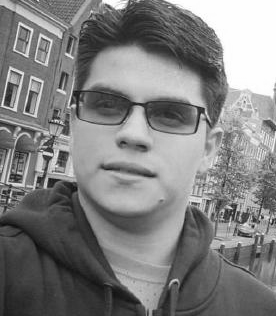
\includegraphics[width=1in,height=1.25in,clip,keepaspectratio]{edilsonphoto}}]{Edilson Galvao} received his computer engineering degree in 2015 from Foundation Center for Analysis, Research and Technological Innovation (FUCAPI) and is pursuing his M.Sc. at UFAM. Currently, he is a Software engineer at Samsung R\&D. His interest is in automated verification and model checking. His work focuses on developing tools for process automation.
\end{IEEEbiography}

\begin{IEEEbiography}
    [{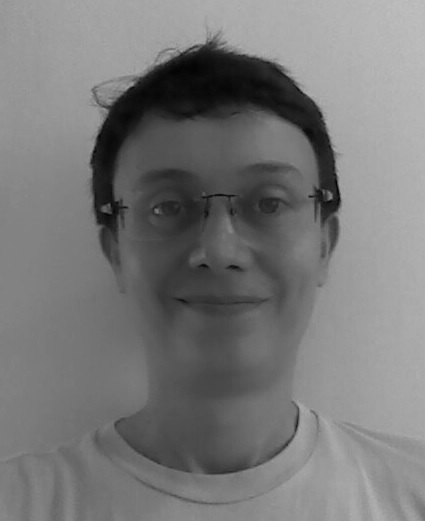
\includegraphics[width=1in,height=1.25in,clip,keepaspectratio]{alessandro3por4_2}}]{Alessandro Trindade}
received his Ph.D. in Computing, BSc and MSc in Electrical Engineering from the Federal University of Amazonas (UFAM) in 2020, 1995, and 2015, respectively. Currently, he holds an Adjunct Professor position in the Electricity Department from UFAM. Before joining UFAM, he worked four years as a renewable energy consultant to the Amazonas State Electric Utility and to the Inter-American Institute for Cooperation on Agriculture (IICA); he also worked for 12 years R\&D and project manager at a non-profit foundation. His interest is in renewable energy, automated verification, and model checking.
\end{IEEEbiography}

\begin{IEEEbiography}
    [{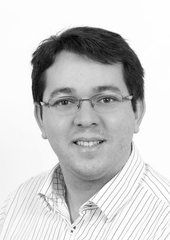
\includegraphics[width=1in,height=1.25in,clip,keepaspectratio]{lucas3por4}}]{Lucas Cordeiro}
received his Ph.D. degree in Computer Science in 2011 from the University of Southampton, UK. Currently, he is a Senior Lecturer in the Department of Computer Science at the University of Manchester, UK, and leads the Systems and Software Verification laboratory. He is also a collaborator in the Postgraduate Program in Electrical Engineering and Informatics at the Federal University of Amazonas (UFAM), Brazil. Before joining the University of Manchester, he worked as a researcher at Oxford University / Diffblue and as an adjunct professor at UFAM; he also worked for six years as a software engineer in the industry. His work focuses on software model checking, automated testing, program synthesis, and embedded \& cyber-physical systems.
\end{IEEEbiography}
% insert where needed to balance the two columns on the last page with
% biographies
%\newpage
%\begin{IEEEbiographynophoto}{Jane Doe}
%Biography text here.
%\end{IEEEbiographynophoto}
% You can push biographies down or up by placing
% a \vfill before or after them. The appropriate
% use of \vfill depends on what kind of text is
% on the last page and whether or not the columns
% are being equalized.
%\vfill
% Can be used to pull up biographies so that the bottom of the last one
% is flush with the other column.
%\enlargethispage{-5in}
% that's all folks
\end{document}
